% -*- latex -*-
%-----------------------------------------------------------------------
%;  Copyright (C) 2015
%;  Associated Universities, Inc. Washington DC, USA.
%;
%;  This program is free software; you can redistribute it and/or
%;  modify it under the terms of the GNU General Public License as
%;  published by the Free Software Foundation; either version 2 of
%;  the License, or (at your option) any later version.
%;
%;  This program is distributed in the hope that it will be useful,
%;  but WITHOUT ANY WARRANTY; without even the implied warranty of
%;  MERCHANTABILITY or FITNESS FOR A PARTICULAR PURPOSE.  See the
%;  GNU General Public License for more details.
%;
%;  You should have received a copy of the GNU General Public
%;  License along with this program; if not, write to the Free
%;  Software Foundation, Inc., 675 Massachusetts Ave, Cambridge,
%;  MA 02139, USA.
%;
%;  Correspondence concerning AIPS should be addressed as follows:
%;          Internet email: aipsmail@nrao.edu.
%;          Postal address: AIPS Project Office
%;                          National Radio Astronomy Observatory
%;                          520 Edgemont Road
%;                          Charlottesville, VA 22903-2475 USA
%-----------------------------------------------------------------------
%Body of final AIPSletter for 31 December 2015

\documentclass[twoside]{article}
\usepackage{graphics}

\newcommand{\AIPRELEASE}{December 31, 2015}
\newcommand{\AIPVOLUME}{Volume XXXV}
\newcommand{\AIPNUMBER}{Number 2}
\newcommand{\RELEASENAME}{{\tt 31DEC15}}
\newcommand{\OLDNAME}{{\tt 31DEC14}}
\newcommand{\NEWNAME}{{\tt 31DEC16}}
\newcommand{\Tsys}{${\rm T}_{\rm sys}$}

%macros and title page format for the \AIPS\ letter.
\input LET98.MAC

\newcommand{\MYSpace}{-11pt}

\normalstyle

\section{General developments in \AIPS}

\subsection{Reduction of VLB, VLA and ALMA data in \AIPS}

\AIPS\ continues to be the main software system for the reduction of
VLBI data from the VLBA and other telescopes.  Since 2010, there have
been numerous improvements to \AIPS\ that enable full calibration of
data from the Karl G. Jansky VLA and most imaging operations as well.
The one exception is the wide-band (bandwidth synthesis) deconvolution
algorithm (``MSMFS'') being developed in \CASA\ by Urvashi Rao
Venkata, for which there is no comparable function in \AIPS\@.
Calibrated $uv$ data may be exported from \AIPS\ in ``UVFITS'' format
for use in that program.  ALMA data may also be reduced in \AIPS,
although the package is not fully qualified to calibrate data from
linearly-polarized feeds.  See Appendix E of the \AIPS\ Cookbook,
available via the \AIPS\ web site, for details.

\subsection{\Aipsletter\ publication}

We have discontinued paper copies of the \Aipsletter\ other than for
libraries and NRAO staff.  The \Aipsletter\ will be available in
PostScript and pdf forms as always from the web site listed above and
will be shipped with all distributions of \AIPS\@.  It will be
announced on the bananas and mnj list servers and, usually, in the
NRAO e-News mailing.

\subsection{Current and future releases}

We have formal \AIPS\ releases on an annual basis.  We recommend a
full binary installation method for both the frozen and development
versions for MacIntosh OS/X (PPC and Intel chips), Solaris, and Linux
(32- and 64-bit) systems, but all architectures can do a full
installation from the source files.  If you develop \AIPS\ code
locally {\it or have system managers that forbid the use of\/} {\tt
  rsync} or {\tt cvs}, you will need to do a source-level
installation.  The current release is called \RELEASENAME\ and is now
``frozen.''  If you took a development copy of this version at some
earlier date, you should use the ``Midnight Job'' (MNJ) to bring it up
to date.  You need to run a MNJ only once in 2016 to convert your copy
of \RELEASENAME\ into the frozen version.  However, when patches to
\RELEASENAME\ are announced in 2016, you may apply them with the
MNJ\@.  This \Aipsletter\ is intended to advise you of corrections and
improvements in this release.

We have begun a new version, called \NEWNAME, which is now under
development by the \AIPS\ Group.  You may fetch and install a complete
copy of this version at any time.  Having fetched \NEWNAME, you may
update your installation whenever you want by running the MNJ\@.  This
uses {\tt cvs}, {\tt rsync}, and/or transaction files to copy all
changed text files and then to copy the binary files or to compile the
code selectively based on the code changes and compilations we have
done.  We expect users to take their source-only or binary version of
\NEWNAME\ \AIPS\ over the Internet (via \emph{anonymous} ftp).  Both
versions require you to copy the installation procedure {\tt
  install.pl} via {\tt ftp}; the source-only version also requires you
to ftp the 125-Mbyte {\tt   \NEWNAME.tar.gz} compressed tar file.
Linux sites will almost certainly have {\tt cvs} installed; other
sites may have installed it along with other GNU tools.  Secondary
MNJs will still be possible using {\tt ssh} or {\tt rcp} or NFS as
with previous releases.  We have found that {\tt cvs} works very well,
although it has one quirk. If a site modifies a file locally, but in
an \AIPS-standard directory, {\tt cvs} will detect the modification
and attempt to reconcile the local version with the NRAO-supplied
version.  This usually produces a file that will not compile or run as
intended.  Use a new name for the task or put a copy of the task and
its help file in a private disk area instead.

\AIPS\ is now copyright \copyright\ 1995 through 2015 by Associated
Universities, Inc., NRAO's parent corporation, but may be made freely
available under the terms of the Free Software Foundation's General
Public License (GPL)\@.  This means that User Agreements are no longer
required, that \AIPS\ may be obtained via anonymous ftp without
contacting NRAO, and that the software may be redistributed (and/or
modified), under certain conditions.  The full text of the GPL can be
found in the \texttt{15JUL95} \Aipsletter\ and is included with every
distribution in file {\tt \$AIPS\_ROOT/{\it release-name}/COPYING}\@.


\subsection{Installing a new version}

If compiling locally, new releases must be installed from the tar ball
for that release.  {\tt 31DEC15} contains improvements to the code
which should make local compilation more reliable.  If using the
binary installation, a full new installation must also be done with
{\tt rsync}.  The {\tt cvs} system used in the MNJ requires this.
When installing a new \AIPS\ release in a system that already has a
previous release, we recommend that {\tt install.pl} be used and that
the previous release be left in place, at least until the new
installation has been verified.  If you do this, then you will not
have to re-edit the disk, printer, and tape lists and can simply skip
all those pages in the {\tt install.pl} menus.  The old {\tt
  \$HOME/.AIPSRC} file may be left in place, but it will need to be
edited.  The lines giving the {\tt DOWNLOADED} and {\tt UNPACKED}
parameters should be cleared and the {\tt CCOMOPT} line should be
changed to point to the current release rather than the previous one.
If you have made a special version of {\tt do\_daily.{\it host}}, you
should preserve it under a new name and restore it after the install.
If you have an odd set of \AIPS\ versions, the {\tt
  \$AIPS\_ROOT/AIPSPATH.*SH} files may need to be edited after the
install to set the desired versions.  The file {\tt
  \$SYSLOCAL/UPDCONFIG} also needs to be edited to correct your e-mail
address(es).

{\tt 31DEC09} contains a change in the format of antenna files.
Previous releases will not understand the antenna coordinates for
arrays that were traditionally left-handed (VLBI primarily).  The
format change occurs automatically when any {\tt 31DEC09} or later
antenna-file specific code reads the file, after which older releases
will have difficulties.  {\tt 31DEC15} contains a change in the
headers of $uv$ data sets which will not be understood by previous
versions.  Note that the only version which we patch for major errors
is \RELEASENAME; even \OLDNAME\ is no longer changed.

\section{Preview of coming attractions}

The \NEWNAME\ release already contains a few changes that we decided
were a bit risky or not needed in \RELEASENAME\@.   The new verb {\tt
  DAYNUMBR} displays the day number in the year for the observation
data of the image or $uv$ file selected.

\vfill\eject
\section{Improvements of interest to users in \RELEASENAME}

We expect to continue publishing the \Aipsletter\ every six months
along with the annual releases.  Significant time was spent in the
last six months on correcting the code to comply with modern
compilers, particularly {\tt gfortran}.  There are a few new tasks and
verbs released in the last six months nonetheless.  {\tt ALVAR} is a
new task to compute and plot the Allan Variance of a $uv$ data set as
a function of the integration time.  The old task by that name was
renamed {\tt ALVPR} to reflect its major printing role.  New tasks
{\tt XG2PL} and {\tt RM2PL} were written to display fit spectra from
{\tt XGAUS} plus {\tt ZEMAN} and from {\tt RMFIT}, respectively.  New
verb {\tt REVERSN} was created to check the actual number of extension
files of specified type present for a cataloged file.

In the first six months of \RELEASENAME\ the new tasks were {\tt
SNFIT} to fit Gaussians to drift-scan gain solutions, {\tt UVFRE} to
re-grid visibility data in frequency space to match a second data set,
{\tt HOLOG} to transform and analyze holography data, {\tt PANEL} to
convert {\tt HOLOG} output to panel adjustment tables, {\tt STACK} to
combine multiple images without regard for coordinates, and {\tt
  TVHLD} to display and save histogram-equalized versions of images.
New verb {\tt TVLAYOUT} also assists in displaying holography results
and new procedure {\tt DOVLAMP} assists in converting EVLA SysPower
data to gains for VLB usage.

Normally, bugs which appear in an \AIPS\ {\tt TST} version and then
are fixed in that same version before its release get little or no
discussion in the \Aipsletter\@.  Since a rather large number of sites
now install the {\tt TST} version of \AIPS\ during its development,
this is somewhat of an oversight.  We urge you to run the ``Midnight
Job'' at least once after \RELEASENAME\ is frozen to bring it up to
date and to fix all bugs of this sort.  We urge active sites to use
the MNJ and, when something odd occurs, to examine {\tt CHANGE.DOC}
using the cgi tool available from the \AIPS\ documentation web page
({\tt http://www.aips.nrao.edu/aipsdoc.html}).  Please do not
hesitate to contact us via the NRAO help desk ({\tt
  https://help.nrao.edu}) or via e-mail {\tt daip@nrao.edu} with any
questions or suspicions that there are problems.

\subsection{UV data}

\subsubsection{New Amplitude Calibration Strategy for the VLBA}

The VLBA utilities ({\tt VLBAUTIL}) and the VLBA reduction pipeline
({\tt VLBARUN}) were changed to incorporate the new amplitude
calibration strategy described by Craig Walker in VLBA Scientific Memo
\#37 ``Flux Density Calibration on the VLBA'' (2015).  Three
procedures were added to {\tt VLBAUTIL}: {\tt VLBACCOR}, {\tt
  VLBABPSS} and {\tt VLBAAMP} to aid in this new strategy.  Also,
several improvements were added to {\tt VLBARUN} in order to have it
behave more robustly.

These changes were made because it was reported that, with the advent
of the Roach Digital Backend (RDBE), there were 10-15\%\ errors in the
amplitudes when compared to the 5\%\ pre-sensitivity upgrade VLBA
observations.  For more information on the RDBE see the VLBA
Observational Status Summary {\tt
(https://science.nrao.edu/facilities/vlba/docs/manuals/oss/sig-path/rdbe)}.
Craig Walker studied this problem and wrote VLBA Scientific Memo \#37
(2015) describing a new VLBA amplitude calibration strategy to counter
this problem.  Three new procedures were added to {\tt VLBAUTIL} to
accommodate this new strategy and {\tt VLBARUN} was modified to use
the new calibration scheme.  This new strategy interleaves the old
{\it a priori} calibration with instrumental delay and complex
bandpass calibration.  So, instead of doing {\tt VLBACALA} ({\tt
  ACCOR}, {\tt APCAL}, and accompanying tasks) and then proceeding
with instrumental delay and bandpass calibration, one performs the
following steps
\begin{description}
\myitem{VLBACCOR}\hspace{3pt} ({\tt ACCOR}): calibrate sampler
      corrections.
\myitem{VLBAPCOR}\hspace{3pt} ({\tt PCCOR}) or {\tt VLBAMPCL} ({\tt
      FRING}): calibrate the instrumental delays.
\myitem{VLBABPSS}\hspace{3pt} ({\tt BPASS}): calibrate complex
      bandpass response function, making sure to normalize by the
      entire band (not just the inner 75\%\ which is the default).
\myitem{VLBAAMP}\hspace{3pt} ({\tt ACSCL} and {\tt APCAL}): apply
      autocorrelation correction (to adjust bandpass normalization)
      and do final amplitude calibration using ${\rm T}_{\rm sys}$ and
      gain curves.
\end{description}

If you have data from before the sensitivity upgrade, this new method
may improve your amplitudes a small amount, but the old strategy
should still work.

\subsubsection{Miscellaneous}

\begin{description}
\myitem{RLDLY} was changed to allow more than one calibration scan and
           to write an {\tt SN} table under all circumstances.  It was
           changed to allow control over the minimum SNR, to limit the
           delays used in averaging, and to display the rms over all
           reference antennas as well as the formal uncertainties.
\myitem{DELZN} was revised to offer the {\tt DISP} opcode to solve for
           dispersion as another $1/\sin({\rm elevation})$ parameter
           allowing it to plot the fit, correct the current {\tt CL}
           table, and write a text file for {\tt CLCOR}.  The help
           file explanation of what is plotted was improved greatly.
\myitem{CLCOR} was given the {\tt DISP} option to correct a {\tt CL}
           table for dispersion as a function of time and elevation.
           The {\tt EOPS} option was tested on EVLA data observed with
           a bad clock and found to work well now that we have a {\tt
           CQ} table.  Messages about ``VLBA only'' were toned down.
\myitem{FITLD} and {\tt UVLOD} were changed to check and correct any
           index tables they might read and create new ones if the
           index table was not present in the FITS file.
\myitem{DBCON} was changed to try to use the incoming index tables to
           define the output scan structure, to correct the output
           frequency ID forms which were confused when there were
           several in the input, and to mark unknown sort orders with
           asterisks.
\myitem{PCAL} died on fully-flagged channels when doing models and
           died on end-of-file when doing {\tt SPECTRAL} false.  It
           also died when sample averages had some but not all
           polarizations flagged.  Corrected the code to handle these
           ``errors'' gracefully.  The XY {\tt SOLTYPE} will be used
           on linearly-polarized data only if {\tt CPARM(5)}$ > 0$\@.
           {\tt APPR} works much better on unpolarized sources even
           with linearly-polarized feeds.
\myitem{EDITA} {\tt EDITR}, and {\tt SNEDT} now offer the {\tt
           DO3COLOR} option to differentiate between IFs and
           polarizations in ``crowded'' displays.  Times at the ends
           of the display were extended outward a bit in the flags.
\myitem{RFLAG} did not allocate enough memory for more than one source
           when doing the {\tt DOSCALE} option.
\myitem{FRING} and {\tt RLDLY} do not work if the increment between
           spectral channels in a group and between IFs in that same
           group have opposite sign.  An error test for this was added
           to both.
\myitem{FLOPM} is the cure for the above issue and acquired a new
           option to flop only IFs, leaving the spectral channel order
           unchanged.
\myitem{ALVAR} is a new task to compute and plot the Allan variance
           from phases or normalized complex visibilities as a
           function of integration time.  The old task, now called
           {\tt ALVPR} prints the Allan Variance at a particular
           integration time separating baselines and IFs.
\myitem{APCAL} computed the spill-over correction improperly due to an
           incorrect call sequence found by {\tt gfortran}.
\myitem{TACOP} was changed to allow flagging of {\tt SN}, {\tt TY},
           and {\tt SY} tables.
\myitem{TYCOP} is the new name for {\tt SYCOP} to reflect its new
           ability to manipulate {\tt TY} tables as well as {\tt SY}
           tables in order to reduce bad values resulting from RFI\@.
\myitem{VPFLG} has an option to flag cross-hand data if one or more
           parallel-hand correlations are flagged as an alternative to
           flagging every polarization if any one is flagged.
\myitem{EVAUV} was given the {\tt SMODEL} option for completeness.
           This allows comparison between a simple user model and the
           data.
\myitem{TYSMO} did not work when the data set contained only one
           polarization.  Corrected pointers to know always that there
           is only one.  The task used the smoothing time for
           ${\rm T}_{\rm sys}$ when it should have used the smoothing
           time for gains.
\myitem{UVFLG} did not re-initialize all internal adverbs in the {\tt
           INTEXT} option and, in particular, messed up a defaulted
           time-range.  Added emphasis in the help file that each flag
           command in {\tt INTEXT} is essentially independent.
\myitem{ATLOD} was corrected to work properly with magnetic tape.
\myitem{UVHOL} can now do scalar averaging over time and antennas and
           can average over moving antennas.  It will do I
           polarization only on lineraly-polarized data.
\myitem{PBEAM} was overhauled to write out the data, model, and
           residual as cataloged image files and to do contour plots
           rather than row/column traces.
\end{description}

\subsection{Analysis}

From some initial user experiences, some of the rough edges in the
spectral-fitting tasks {\tt XGAUS}, {\tt ZEMAN} and {\tt RMFIT} have
been addressed.  In particular, all three now make the work tables
over the full input images.  Adverbs {\tt BLC(1)} and {\tt TRC(1)} are
still used to control the spectral channels over which peak fluxes are
found and so should probably be set to eliminate only bad edge
channels if any.  {\tt BLC(2)}, {\tt BLC{3}}, {\tt TRC(2)}, and {\tt
  TRC(3)} now only control the region over which the fit is done in
the present execution.  Since the images may now be large, all three
tasks were given {\tt SET WINDOW} and {\tt RESET WINDOW} options in
the image editing phase.  The sub-images are blown up to fit the screen
for easy viewing.  The spectral baseline guess in {\tt XGAUS} is now
always zero and confusing adverbs {\tt BCHAN} and {\tt ECHAN} are
gone.  This works much better in most cases.  {\tt OUTSEQ = 0} now
works as expected with the many output images getting a new sequence
number even if they are not all the same.  The output of images did
not work properly in {\tt RMFIT}\@.  The setting of flags was fixed to
allow all parameter images to be written and the computation of the
uncertainties in the output {\tt Q0} and {\tt U0} images was
corrected.

In support of these tasks, two new tasks were written.  {\tt XG2PL}
makes a plot file of the {\tt XGAUS} solution for a selected pixel or
the average over a circular or rectangular region.  The fit from {\tt
  ZEMAN} for the same pixel or region may be included as a lower panel
in the plot.  {\tt RM2PL} was written to make similar plots of the
{\tt Q} and {\tt U} solutions found by {\tt RMFIT}\@.  \AIPS\ Memo 118
(see below) was updated to describe all of these changes and additions.

\begin{description}
\myitem{IRING} used an incorrect geometry formula when figuring out
           the annulus to assign to each pixel when the inclination
           was not zero.
\myitem{PATGN} was given the option {\tt INVB} to write out 1.0
           divided by the primary beam.
\myitem{MATHS} was given the {\tt DIVP} option to output a polynomial
           in 1.0 over the input image values.
\myitem{NINER} operation {\tt KRSH} did only 4 of the 8 matrix cases
           and then required the data values to be greater than 1.0.
           Corrected the handling of the matrices and to allow any
           data values to be returned.
\myitem{BLANK} operation {\tt FLUW} actually flagged all pixels less
           than {\tt DPARM(3)} which is really operation {\tt SELC} at
           least in part.  Changed to access the code that correctly
           implements this operation (window set by flux).
\myitem{RMSD} was corrected to handle fully-blanked regions and to
           limit excessive verbiage.  The robust method works better
           than the histogram.
\myitem{MFPRT} was changed to allow a wider range of scales and to
           apply {\tt FLUX} to the beam-corrected total flux
\myitem{OMFIT} had some Fortran errors corrected and the default for
           {\tt NOISE(1)} was changed to 1.0, which means the weights
           are correctly calibrated.  The help file was changed to
           clarify the meaning of this adverb and its consequences in
           the reported solution rms.
\myitem{Tests} on units of brightness were changed in numerous tasks
           to avoid case sensitivity; {\tt CASA} uses mixed case (\eg\
           {\tt Jy/beam}).
\end{description}

\vfill\eject
\subsection{General: Miscellaneous}

Apple has released a new version of its operating system numbered
10.11 and called ``El Capitan.''  This change affects various things
in software systems in the general interest of increasing security.
\AIPS\ binary distribution has depended on setting a library path to
point at the Intel compiler run-time libraries.  This is no longer
allowed.  A new script was written {\tt fix\_aips\_elcap.sh} which is
to be run under bash with {\tt sudo} privilege.  It makes links in
{\tt /usr/local/lib} to the needed libraries and then \AIPS\ programs
may be run.  This script needs to be executed, in a separate window,
near the end of running {\tt perl install.pl -n}.  {\tt install.pl}
was revised to copy the script to {\tt \$AIPS\_ROOT} and {\tt
  \$SYSLOCAL} and then pause to allow the user to run the script in
that separate window.

{\tt install.pl} was also revised after watching numerous new users
install \AIPS\@.  The user is now repeatedly warned about putting
blanks in {\tt \$AIPS\_ROOT} and paths to data areas and told not to
use {\tt NRAO} or {\tt OARN} in site names.  If no data area was
specified, the suggested area is now created for the user.  At the
end, numerous added and highlighted messages appear about system
services and, for Macs, about {\tt /etc/sysctl.conf}.  ``Laptop'' is
now defaulted to true with a highlighted warning about the change.

Verbs {\tt PRTHI} and {\tt PRTMSG} can produce a great deal of paper
accidentally when directed straight to a line printer.  They were
changed to count the number of lines about to be printed and to ask
the user for confirmation if the number of lines exceeds 400.  Let's
save a tree!  On occasion, the catalog header may lose track of how
many extensions there are of some type.  \AIPS\ program error or
outside user programs may cause this.  An verb {\tt REVERSN} was
written to examine the disk contents to determine the maximum
extension number of a given extension type and catalog entry there
might be.

The \Cookbook\ was also given attention late in 2015.  A number of
minor changes were made throughout to describe the items in this and
the previous \Aipsletter\@.  In addition, some less commonly used
items, particularly magnetic tape, were de-emphasized.  The VLBI
chapter 9 and Appendix C were overhauled to describe the significant
changes made to VLB utility procedures ({\tt VLBAUTIL}) and the data
reduction pipeline ({\tt VLBARUN})\@.

\subsection{General: Fortran compilers}

The binary distributions of \AIPS\ are compiled with various older
versions of compilers from Intel.  People wishing to develop new
\AIPS\ tasks, or variants of existing \AIPS\ tasks, have limited
choices.  They can ask us to compile and link a task for them, making
the binary available on an anonymous ftp site.  That works for
well-tested programs, but is not appropriate for developing code.
Since the versions of Intel compilers we use are no longer available,
the only other alternative is to obtain a compiler and compile all of
\AIPS\ locally.  The usual choice of compiler is {\tt gfortran} plus
{\tt gcc} from gnu.  Unfortunately, until recently, that has not
worked well.

One of the reasons for the failures was the use of ``automatic''
variables, namely local variables that do not retain their value
between invocations of the subroutine.  The traditional compiler
option {\tt -fno-automatic} to prevent this is honored by some
versions of {\tt gfortran}, but not all.  The {\tt man} pages for {\tt
  gfortran} claim that this option is present even when it is not, but
no {\tt gfortran --help} will admit to it.  Therefore, considerable
effort has been expended to identify variables that need to be {\tt
  SAVE}d in order to retain their values between calls to the routine.
Undoubtedly, more will be discovered later, so your editor's personal
version of \AIPS\ has been compiled with automatic variables allowed.
It was also discovered that automatic allocation of largish buffers
(\eg\ 1.5 Mbytes) can be horribly slow when that buffer is used a
great deal (\eg\ in the data reading routine of the calibration
package).  It was found, however, after the large buffers were {\tt
  SAVE}d, that a version with automatic variables completed the {\tt
  Y2K} test about 10\%\ faster than the same compiler with no
automatic variables.

Another reason for the failures was an interaction between {\tt
  gfortran} optimization and the dynamic allocation of memory for the
pseudo-array processor.  Modern {\tt gfortran} versions do something
bad when optimizing the ``{\tt Q}'' routines, but work well if that
memory is a fixed amount.  Therefore {\tt \$INC/PAPC.INC} was changed
to allow the choice of dynamic or fixed memory to be made before
compiling \AIPS\@.  Another oddity that appeared connected with this
was an apparent limitation of labeled {\tt COMMON}s to a combined
total of 2 Gbytes even in 64-bit versions.  That still allows a
mammoth pseudo-AP of say 200 million double-precision words.  {\tt
  gfortran} also handles the reading of an end-of-file in a Fortran
text file differently from {\tt g77} and has different options for the
{\tt OPEN} command.  {\tt ZTXOP2} was changed to handle this for both
compilers.

Yet another issue has been the alignment of labeled {\tt COMMON}s.
Earlier Fortrans started each labeled {\tt COMMON} block on a double
precision address and we made sure that all double precision variables
appeared first in the list of variables in each {\tt COMMON} block.
Now, {\tt gfortran} starts each labeled {\tt COMMON} block on a
single-precision address unless every declaration of that block
contains explicitly a double-precision variable at its start.  A bad
habit of declaring an image header in its integer form in the local
include and then equivalencing it later to its floating and
double-precision versions causes a misalignment of the {\tt COMMON}\@.
It is best repaired by declaring the double-precision equivalence in
the local include block.

The various versions of {\tt gfortran} produce a plethora of warning
messages.  These were reviewed in detail and many routines were
altered to eliminate unused statement labels, variables, {\tt
  FORMAT}s, and the like.  This review also identified real errors
including {\tt NINER} operation {\tt KRSH}, {\tt IMAGR} when making a
second copy of the data for filtering, {\tt APCAL} when computing the
spill-over correction, {\tt TYSMO} when smoothing gains, and {\tt
  BLANK} operation {\tt FLUW}\@.

\section{Recent \AIPS\ Memoranda}

All \AIPS\ Memoranda are available from the \AIPS\ home page.  \AIPS\
Memo 118 describing \AIPS' spectral fitting was enhance with
descriptions of the new plot tasks {\tt XG2PL} and {\tt RM2PL}\@.

\begin{tabular}{lp{5.8in}}
{\bf 118} & {\bf Modeling Spectral Cubes in \AIPS}\\
   &  Eric W. Greisen, NRAO\\
   &  June 19, 2014, {\it revised September 16, 2015}\\
   &   \AIPS\ has done Gaussian fitting along the $x$-axis of image
   cubes with task {\tt XGAUS} since the 1980s.  That task has
   recently been overhauled to be much easier to use and much more
   capable.  In like fashion, new tasks {\tt ZEMAN} and {\tt RMFIT}
   have been developed.  The former fits the standard leakage and
   scaling terms for Stokes V cubes, including a new option to do this
   for each of the Gaussians found by {\tt XGAUS}\@.  The latter fits
   polarization models to Stokes Q and U cubes, using the output of
   Faraday Rotation Measure Synthesis (\AIPS\ task {\tt FARS}) to
   assist with initial guesses.  The models can contain multiple
   components each with a polarization flux, angle, rotation measure,
   and rotation measure ``thickness.''  The present memo describes the
   functions of these tasks in some detail with numerous graphical
   examples.  This memo also discusses two new tasks to plot spectra
   with model fits and a number of tasks which make visibility and
   image model files.
\end{tabular}

\vfill\eject
\section{Patch Distribution for \OLDNAME}

Because of the extensive use of binary installations, we now patch the
master copy of the most recently frozen version.  Older versions are
not corrected even for egregious errors.  Thus, \OLDNAME\ was patched
during 2015 and \RELEASENAME\ will be patched as needed during 2016.
Your copy of them may be corrected simply by running a Midnight Job.
Information about patches and the code may be found using links from
the main \AIPS\ web page or by  {\it anonymous} \ftp\ to the NRAO
server {\tt ftp.aoc.nrao.edu}.  Documentation about patches to a
release is placed on this site at {\tt pub/software/aips/}{\it
  release-name} and the code is placed in suitable sub-directories
below this.  Patches to older releases are kept here as well, but they
will require local compilation.

The \OLDNAME\ release is no longer available for installation and will
no longer receive patches even for egregious errors.  It had a number
of important patches during 2015.  They are
\begin{enumerate}
   \item\ {\tt DOFARS} procedure and inputs retained adverbs no longer
          used by {\tt FARS}. {\it 2015-01-02}
   \item\ {\tt RMFIT} failed to copy the {\tt FQ} table to the output
          residual images. {\it 2015-01-13}
   \item\ {\tt FTFLG} messed up antenna numbers in the output {\tt FG}
          table when a single antenna or baseline was used.
          {\it 2015-01-16}
   \item\ {\tt VLBATECR} had trouble around the end of the year
          deciding what files needed to be downloaded. {\it
            2015-01-19}
   \item\ {\tt VLBARUN} requires {\tt convert} to make the html output
          files.  Added tests and a control on {\tt DOTV}.
          {\it 2015-01-19}
   \item\ {\tt BPASS} had an array and history writing code which
          could not handle more than 32 antennas. {\it 2015-01-20}
   \item\ {\tt MORIF} messed up bandpass and other spectral tables.
          {\it 2015-01-29}
   \item\ {\tt TYSMO} did not apply clipping unless median-window
          filtering was also requested. {\it 2015-02-11}
   \item\ {\tt BPASS} did not understand that low-level VLB routines
          expected left-handed antenna coordinates.
          {\it 2015-02-21}
   \item\ UV data disk I/O had an issue if the full file fit into the
          first of the two buffers and the disk file was exactly the
          right size! {\it 2015-04-24}
   \item\ {\tt START\_AIPS, START\_TVSERVERS} needed a grammar change to
          support Mac Yosemite systems. {\it 2015-04-24}
   \item\ Basic calibration subroutines mis-computed the channel
          wavelengths and did not always do the dispersion correction.
          {\it 2015-05-19}
   \item\ {\tt XAS} needed a change to support Mac Yosemite systems
          and also to write black character backgrounds.
          {\it 2015-05-20}
   \item\ {\tt KRING} help file adverb list did not match that of the
          Fortran. {\it 2015-06-17}
   \item\ {\tt IMAGR} did not do the baseline-based time averaging
          properly for the last samples written to the work file.
          {\it 2015-06-22}
   \item\ {\tt PCAL} did not detect fully flagged channels when using
          a source model and so died.  {\it 2015-08-14}
   \item\ {\tt SETJY} had bad formats capable of aborting the task.
          {\it 2015-08-22}
   \item\ {\tt SAD} and {\tt TVSAD} hid the new model-fit table when
          making a stars table.  {\it 2015-09-07}
   \item\ {\tt PCAL} did not do mode {\tt SPECTRAL = FALSE} correctly,
          leaving files open and then quitting. {\it 2015-09-14}
\end{enumerate}


%\vfill\eject
\section{\AIPS\ Distribution}

From the NRAO system logs, we count apparent MNJ accesses, downloads
of the tar balls, and {\tt rsync} accesses by unique IP address.
Since DSL and some university and other connections may be assigned
different IP addresses at different times, this will be a bit of an
over-estimate of actual sites.  However, a single IP address is often
used to provide \AIPS\ to a number of computers, so these numbers are
at the same time an under-estimate of the number of computers running
current versions of \AIPS\@.  In 2015, a total of 309 different IP
addresses downloaded the frozen form of \OLDNAME\ and 1104 IP
addresses downloaded \RELEASENAME\ in tarball or binary form.  Fully
1070 IP addresses accessed the NRAO cvs master.  Each of these has at
least installed some version of \AIPS\ and 364 appear to have run the
MNJ at least occasionally.  The total number of unique IP addresses in
these three lists was 1817.  The {\tt TST} and cvs numbers are a bit
ahead of last year due mainly to an interferometry school held in
Europe (see plot below).  The other numbers are marginally behind last
year.  The table below shows these numbers as a function of year since
we began recording them.  The attached figure shows the cumulative
number of unique sites, cvs access sites, and download sites known to
us as a function of week in 2015.  The numbers for 2014 are also
plotted and show an increase in 2015 for {\tt TST} and {\tt cvs}, but
a decrease for {\tt NEW}\@.

\begin{center}
\begin{tabular}{|rrrrrrrrr|}
\hline
%year & {\tt TST} name & {\tt NEW} name & \hspace{1em}{\tt TST} &
% \hspace{1em}{\tt NEW} & {\tt TST binary} & {\tt NEW} binary &
% \hspace{1em}{\tt cvs} & Total unique \\
 & & & & & {\tt TST} & {\tt NEW} & & Total \\
\noalign{\vspace{-1mm}}
year & {\tt TST} name & {\tt NEW} name & \hspace{1em}{\tt TST} &
 \hspace{1em}{\tt NEW} & binary & binary &
 \hspace{1em}{\tt cvs} & unique \\
\hline
2004 & {\tt 31DEC04} & {\tt 31DEC03} &  808 & 196 &      &     &  797
 & 1276 \\
2005 & {\tt 31DEC05} & {\tt 31DEC04} &  832 & 246 &  299 &  48 &  982
 & 1460 \\
2006 & {\tt 31DEC06} & {\tt 31DEC05} &  806 & 191 &  402 &  94 & 1050
 & 1398 \\
2007 & {\tt 31DEC07} & {\tt 31DEC06} &  965 & 277 &  669 & 161 & 1385
 & 1811 \\
2008 & {\tt 31DEC08} & {\tt 31DEC07} & 1058 & 246 &  986 & 303 & 1667
 & 2107 \\
2009 & {\tt 31DEC09} & {\tt 31DEC08} & 1228 & 307 & 1082 & 478 & 1855
 & 2399 \\
2010 & {\tt 31DEC10} & {\tt 31DEC09} & 1228 & 307 & 1203 & 477 & 1914
 & 2416 \\
2011 & {\tt 31DEC11} & {\tt 31DEC10} & 1105 & 270 & 1064 & 424 & 1747
 & 2228 \\
2012 & {\tt 31DEC12} & {\tt 31DEC11} &  940 & 284 & 1028 & 396 & 1309
 & 1698 \\
2013 & {\tt 31DEC13} & {\tt 31DEC12} & 1014 & 307 &  990 & 443 & 1264
 & 1937 \\
2014 & {\tt 31DEC14} & {\tt 31DEC13} & 1045 & 333 &  848 & 431 & 1023
 & 1843 \\
2015 & {\tt 31DEC15} & {\tt 31DEC14} & 1104 & 309 & 1001 & 350 & 1070
 & 1817 \\
\hline
\end{tabular}
\end{center}
\vfill
\centerline{\resizebox{!}{4.1in}{\includegraphics{FIG/TWOYEAR.eps}}}
\eject

% Order form and mailer page
%\cleardoublepage
\pagestyle{empty}
%\vfill
%\centerline{\resizebox{!}{23.3cm}{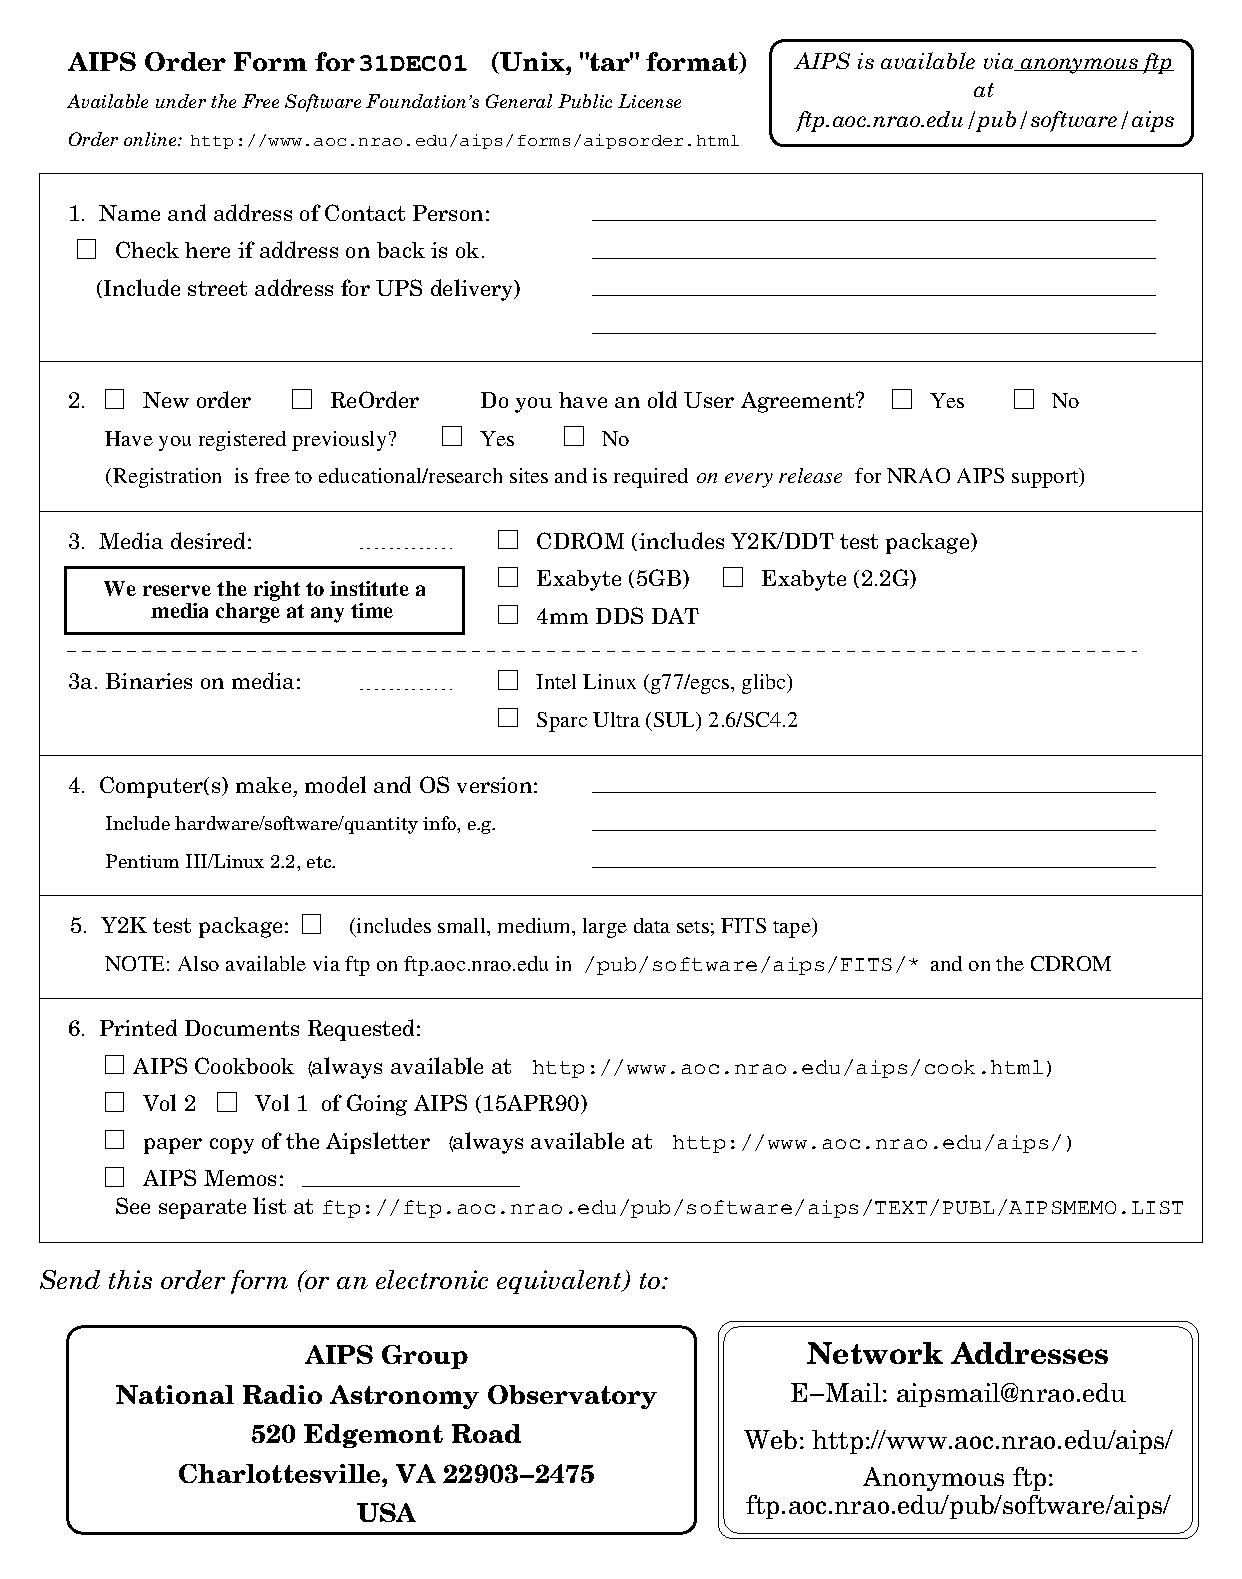
\includegraphics{FIG/AIPSORDER.PS}}}
\vfill\eject
\vbox to 4.4in{
\vspace{12pt}
%\centerline{\rotatebox{-90}{\resizebox{!}{3.5in}{%
%\includegraphics{FIG/Mandrill.color.plt}}}}
\centerline{\resizebox{!}{3.5in}{\includegraphics{FIG/Mandrill.eps}}}
\vspace{12pt}
\centerline{{\huge \tt \AIPRELEASE}}
\vspace{12pt}
\vfill}
\phantom{...}
\centerline{\resizebox{!}{!}{\includegraphics{FIG/AIPSLETS.PS}}}

\end{document}

